% id: 0624
% book: RPM 중3-2 수학 · 06 상관관계
% section: 유형 03 산점도의 이해 (1)
% figure: crop:fig-0624.png
% answer: $35\mkern3mu \%$
% answer_source: 답지
% variant_level: 0 (원본 전사)
% 이 파일은 build.mjs 가 items.json 에서 만든다. 고칠 때는 items.json 을 고친다.
\smash{\raisebox{1.5mm}{\dmkichul{서술형}}}
\noindent\begin{minipage}[t]{0.58\linewidth}\vspace{0pt}\raggedright 오른쪽 그림은 현진이네 반 학생 20명의 수학 점수와 과학 점수에 대한 산점도이다. 수학 점수가 과학 점수보다 높은 학생은 전체의 몇 $\%$인지 구하시오.\end{minipage}\hfill\begin{minipage}[t]{0.4\linewidth}\vspace{0pt}\centering \setlength{\dmfigw}{99.5pt}\ifdim\dmfigw>\linewidth\setlength{\dmfigw}{\linewidth}\fi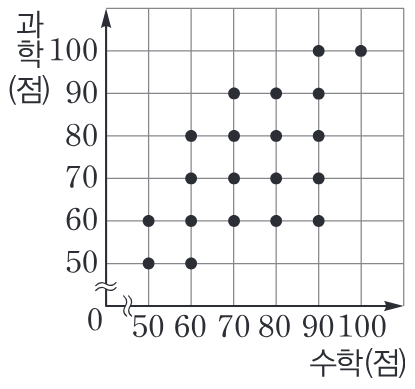
\includegraphics[width=\dmfigw]{figures/fig-0624.png}\end{minipage}\par
